\begin{figure}[!htb]
  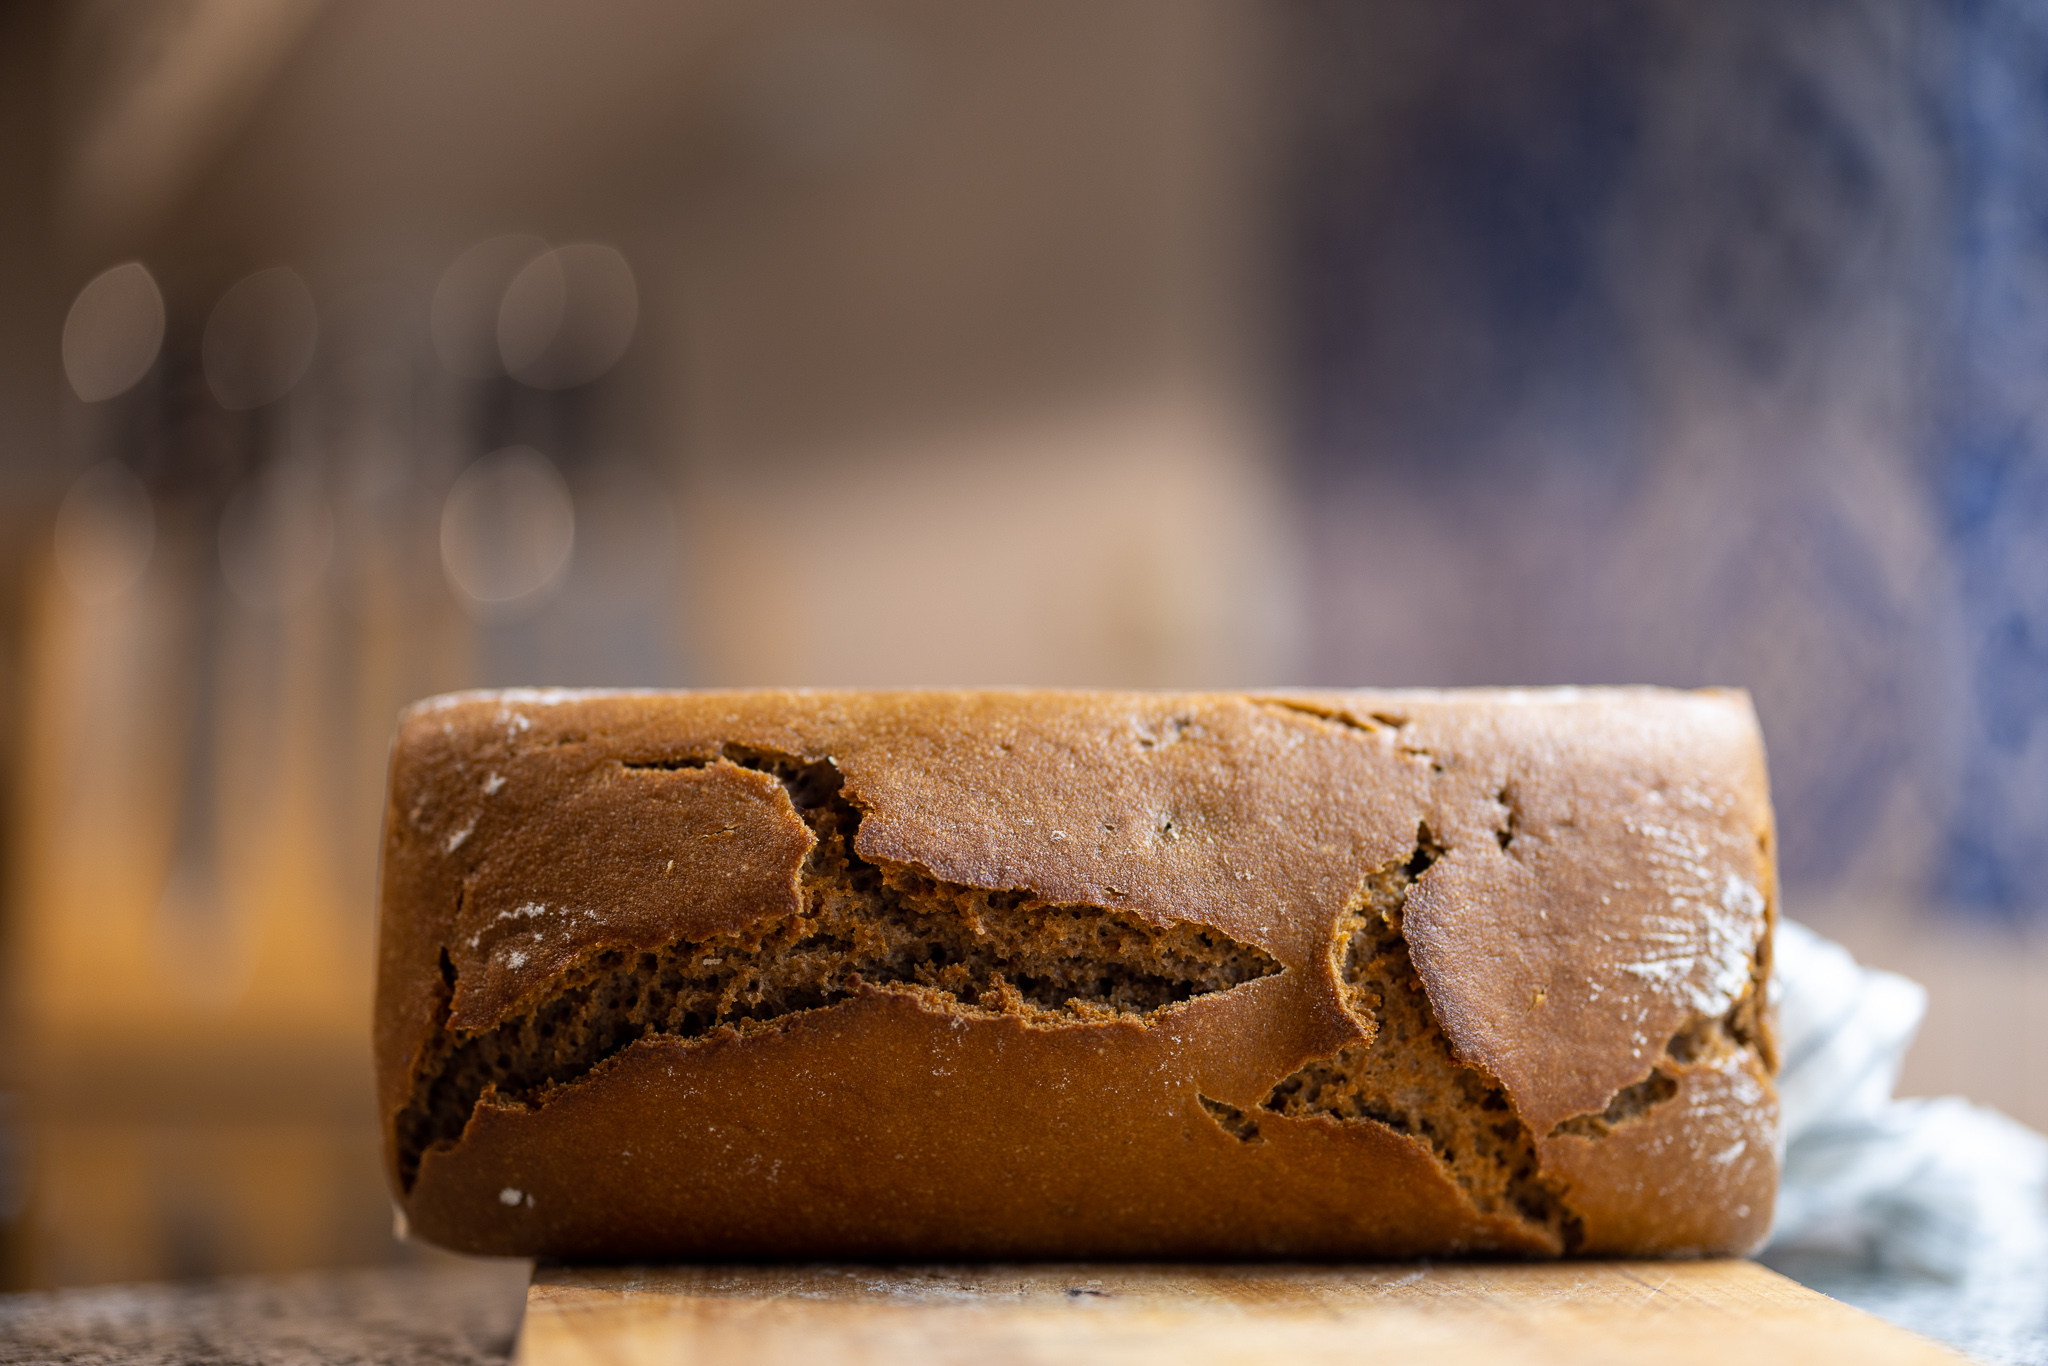
\includegraphics[width=\textwidth]{final-bread}
  \caption{A sourdough rye bread made using a loaf pan. The
  rye bread is not scored. The crust typically cracks
  open during baking.}%
  \label{fig:non-wheat-final-bread}
\end{figure}

In this chapter you will learn how to make a basic sourdough bread
using non-wheat flour. This includes all flour except spelt.
The key difference between wheat and non-wheat flour is
the quantity of gluten. Wheat and spelt feature a high amount
of gluten. The non-wheat flours do not. In the case of rye flour,
sugars called pentosans prevent gluten bonds from properly
forming~\cite{rye+pentosans}.

For these flours including rye, emmer, and einkorn, no gluten
development has to be done. This means there is no kneading,
no over-fermentation, and no issues with making flat bread.
The whole process
is a lot easier. You mix the ingredients and
wait for a certain period until the dough has
reached the level of acidity that you like. Afterward, you
shape the dough or pour it into a loaf pan. After a short proofing
period, the bread can be baked. Due to the lack
of gluten development, the final bread will feature a denser
crumb compared to wheat.

\begin{figure}[!htb]
  \includegraphics{figures/fig-non-wheat-process.pdf}
  \caption{A visualization of the process to make non-wheat sourdough bread.
  The process is much simpler than making wheat sourdough bread. There is
  no gluten development. The ingredients are simply mixed together.}%
  \label{fig:non-wheat-sourdough}
\end{figure}

This chapter will focus on making rye bread. The flour could
be replaced with einkorn or emmer based on your preference.

The following recipe will make you 2 loaves:
\begin{itemize}
  \item 1000 g of whole rye flour
  \item 800 g of room temperature water (80 percent)
  \item 200 g of sourdough starter (20 percent)
  \item 20 g of salt (2 percent)
\end{itemize}

The sourdough starter can be in an active or inactive state. If it has been
at room temperature for a week with no feedings then it will be okay, or 
if it has come right out of the fridge then still it will be no problem.
The dough is very forgiving.

If you follow the suggested dough from the recipe you are making a relatively
wet rye dough. It's so wet that it can only be made using a loaf pan. If
you want to make a freestanding rye bread, consider reducing the hydration
to around 60 percent.

\begin{figure}[!htb]
  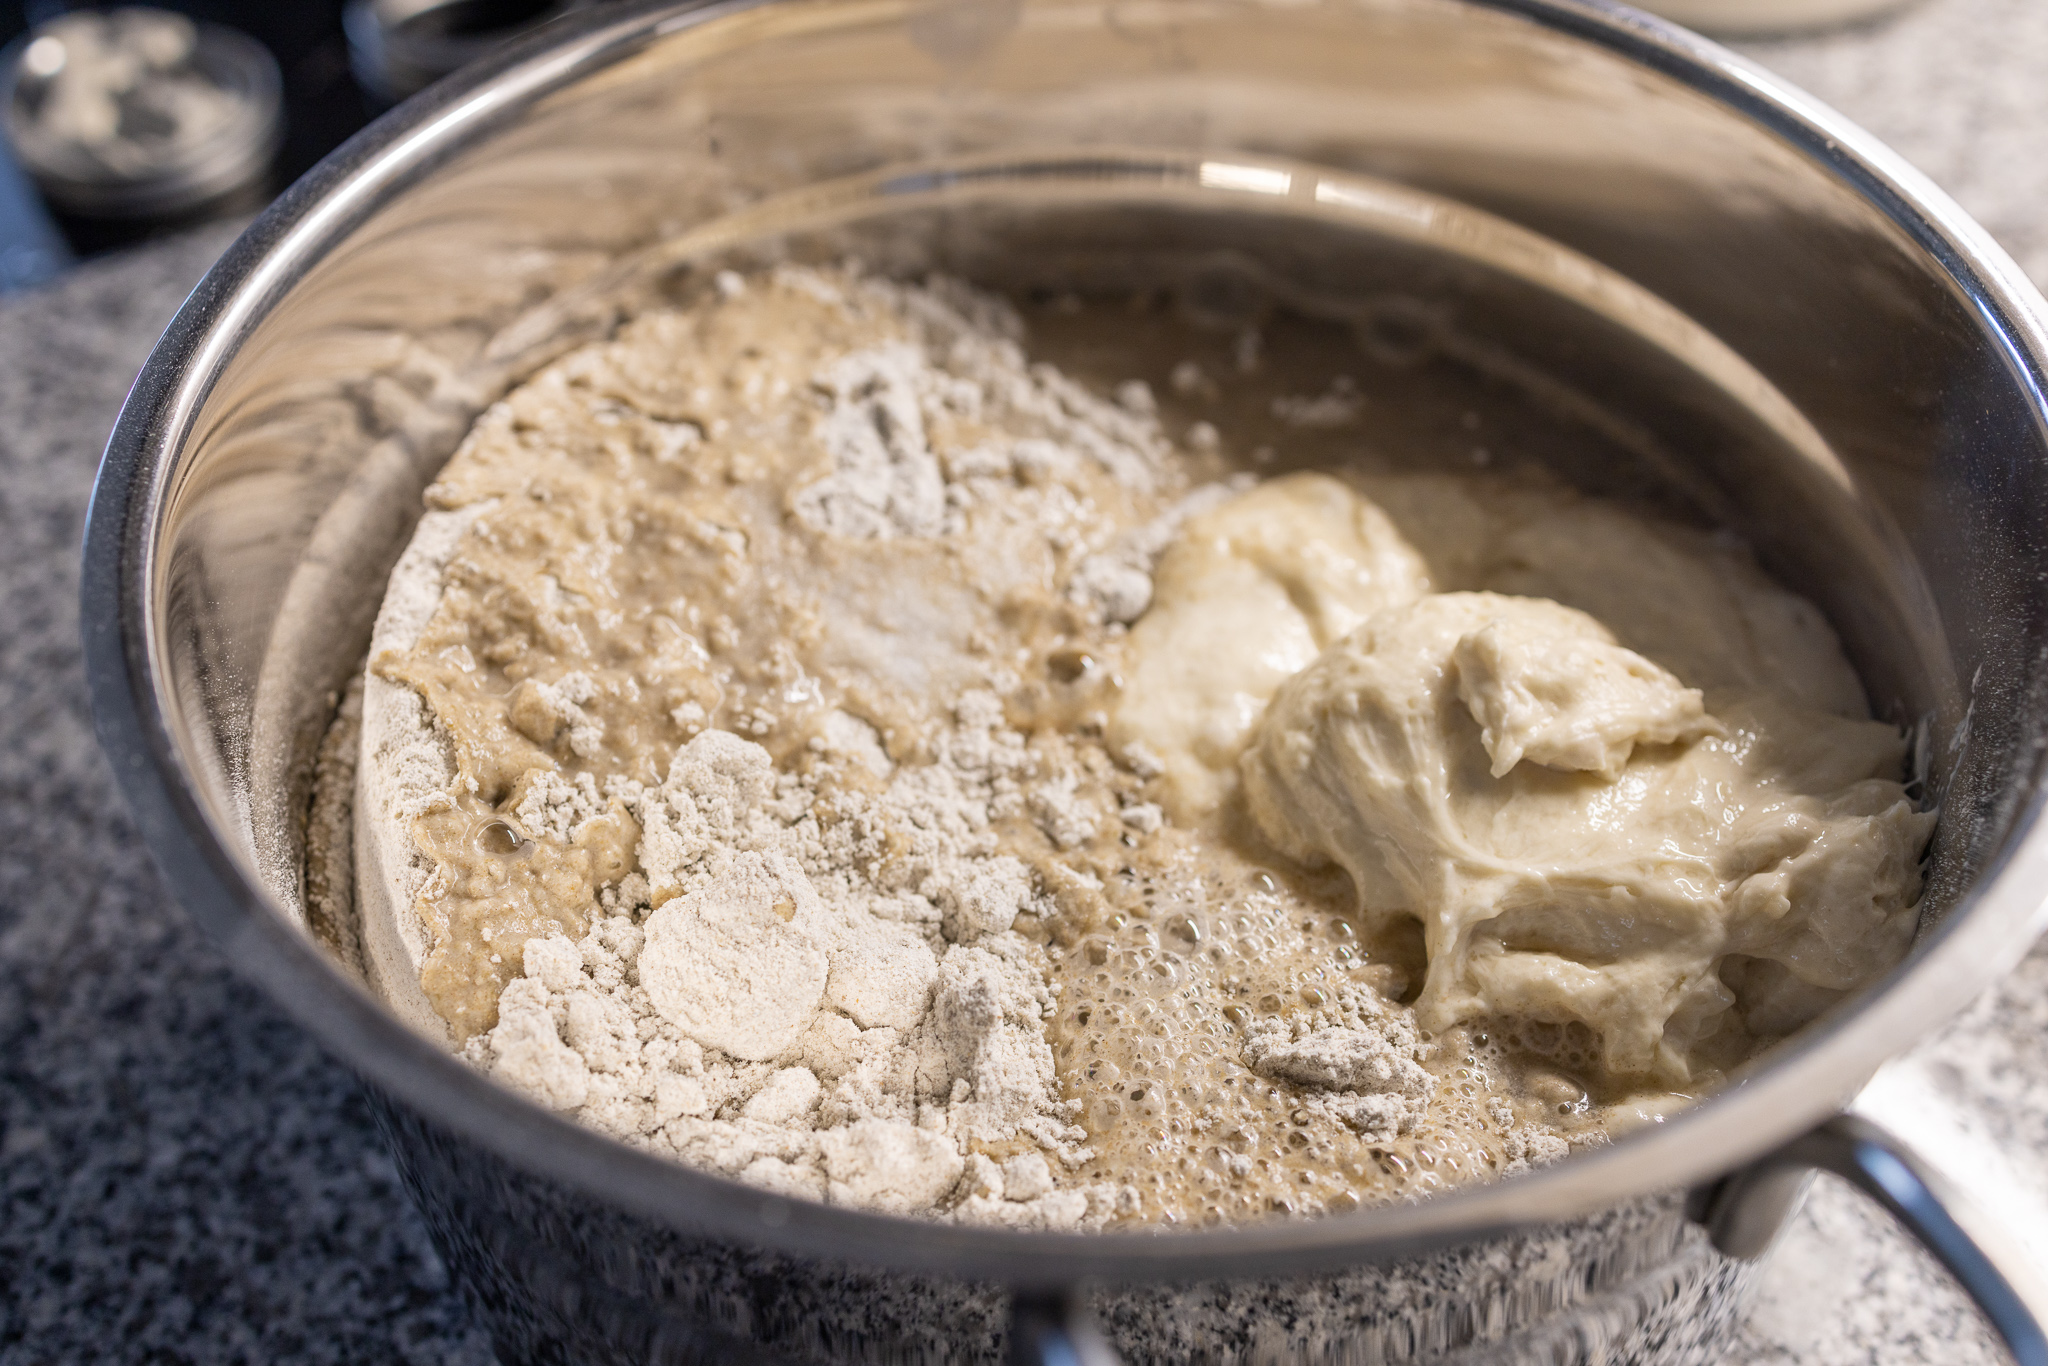
\includegraphics[width=\textwidth]{ingredients}
  \caption{For non-wheat dough the ingredients are mixed together. There is no need
  to develop any dough strength. This simplifies the whole bread-making
  process.}%
  \label{fig:non-wheat-ingredients}
\end{figure}

Mix together all the ingredients with your hands. You can also
opt for a spatula to simplify things. Rye flour itself is very
sticky and unpleasant to mix by hand. The dough will stick
a lot to your hands. If you use a stiff starter, it can be
easier to dissolve it in the dough's water. Once dissolved,
add the other ingredients.

\begin{figure}[!htb]
  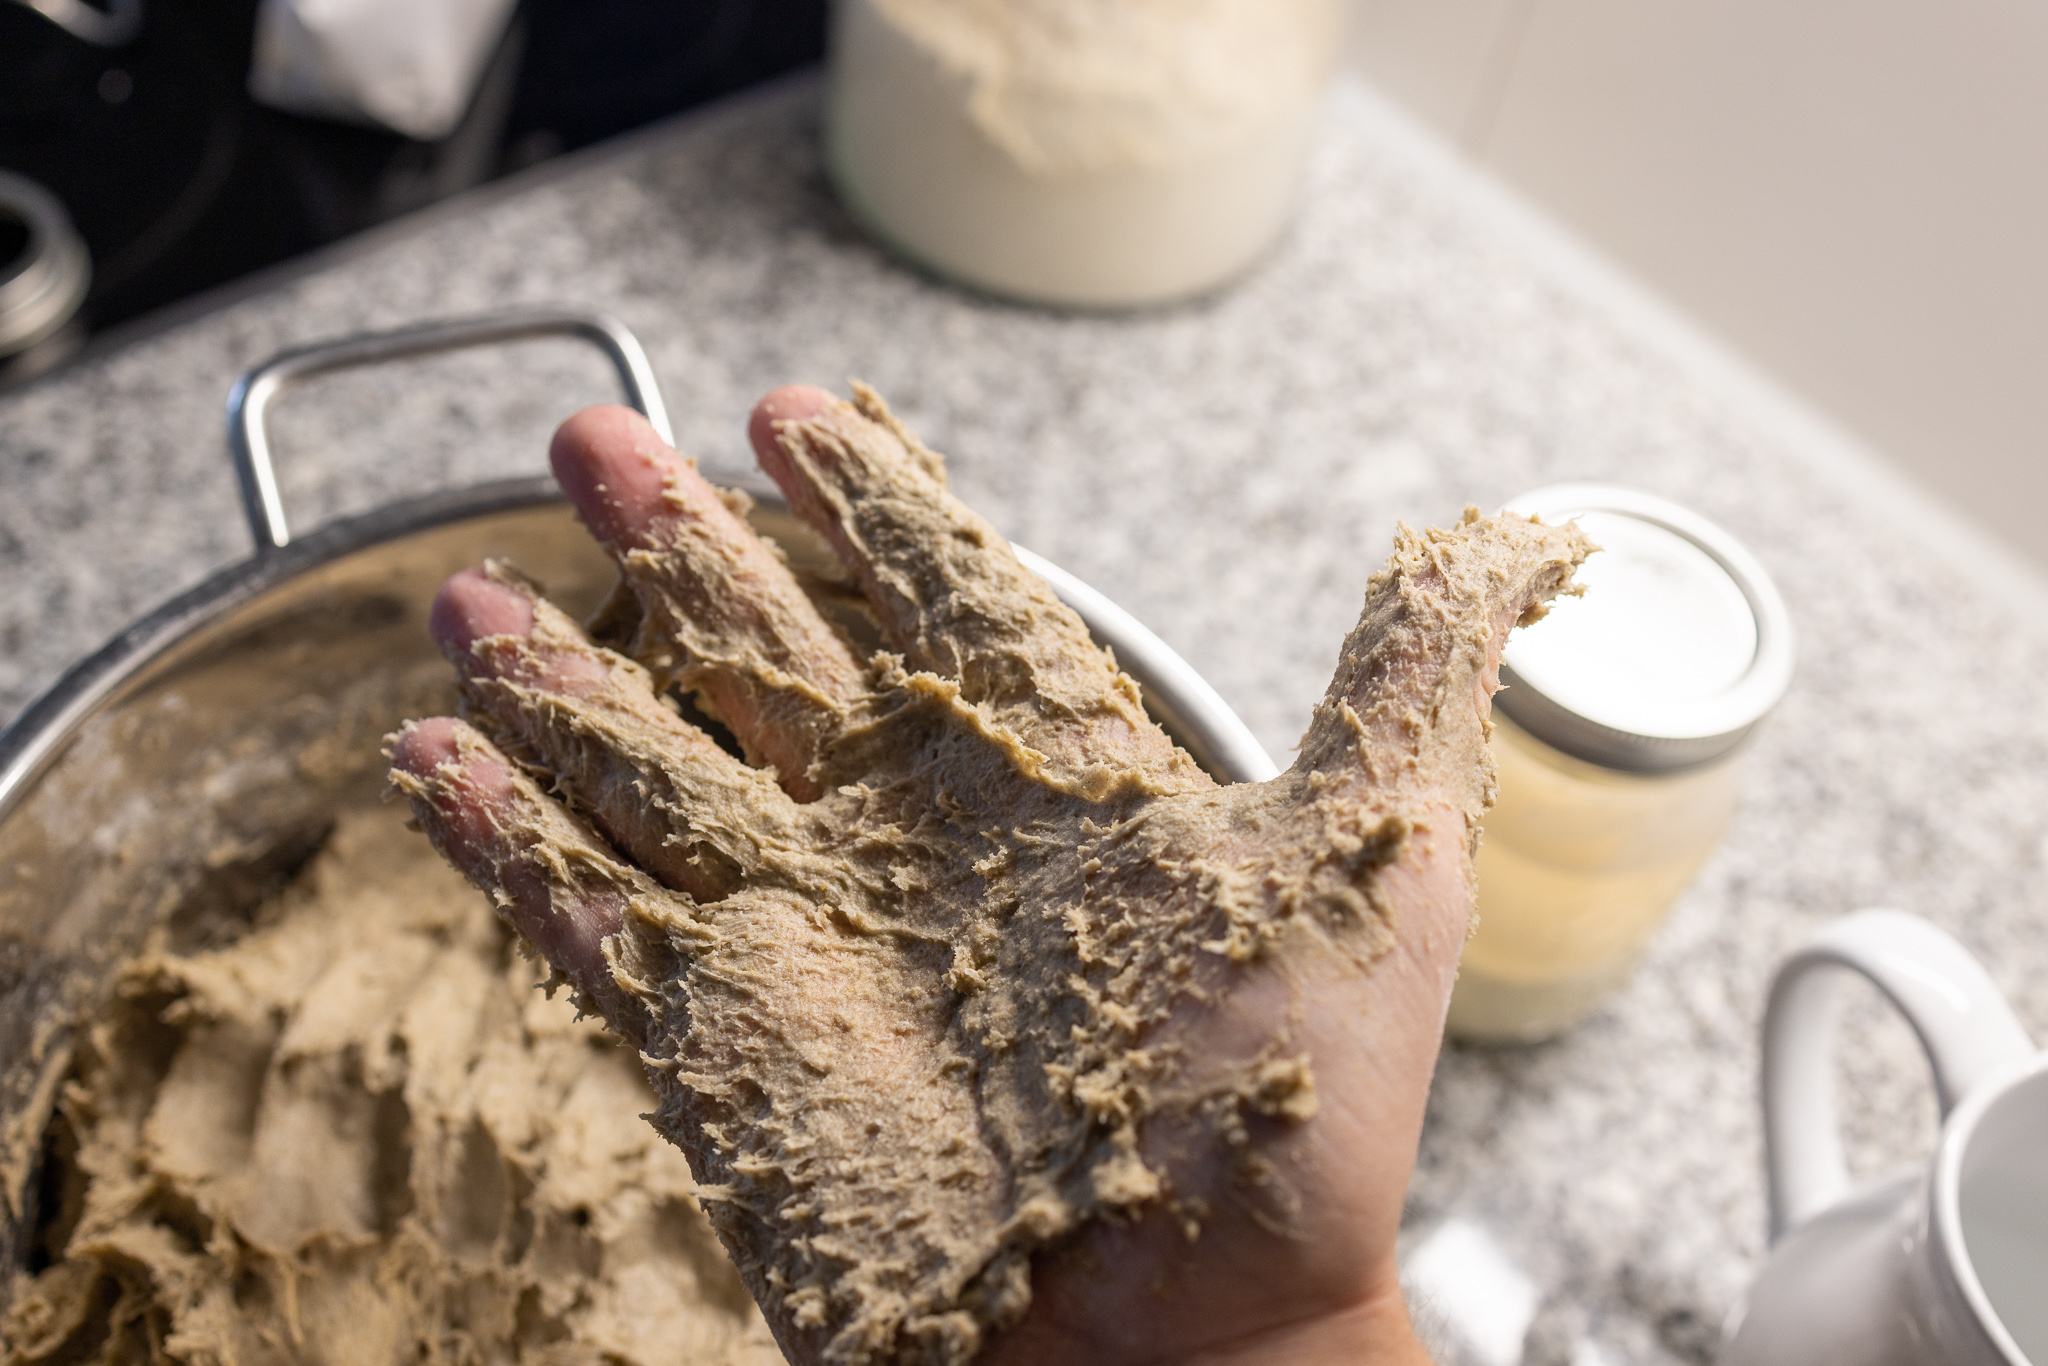
\includegraphics[width=\textwidth]{sticky-hands}
  \caption{Rye flour has a sugar molecule known as pentosan. These pentosans prevent
  the rye flour from building gluten bonds. As a result the dough never features an
  open crumb and is always very sticky when hand mixing.}%
  \label{fig:non-wheat-sticky-hands}
\end{figure}

The goal of the mixing process is to homogenize the dough. There
is no need to develop any dough strength. Once you see that
your sourdough starter has been properly incorporated, your
dough is ready to begin bulk fermentation.

You can bulk ferment the dough for a few hours up to
weeks. By extending the bulk fermentation time, you increase
the acidity the final loaf is going to feature. After around
48 hours, the acidity will no longer increase. This is because
most of the nutrients have been eaten by your microorganisms.
You could let your dough sit for longer, but it wouldn't alter the
final flavor profile by much.

I~recommend waiting until the dough has roughly increased by
50 percent in size. If you are daring, you can taste the dough
to get an idea of the acidity profile. The dough will likely
taste very sour. However, a lot of the acid will evaporate
during the baking process. So the final loaf will not be
as sour as the dough you are tasting.

Once you are happy with the acidity level, proceed to dividing
and shaping your dough. Shaping might not be possible if you opt
for the wetter dough. If you made a drier dough, use as much
flour as needed to dry the dough a little bit and form a dough ball.
There is no folding the dough. All you do is tuck it together
as much as is needed to apply the shape of your banneton.
For the wetter dough, use a spatula and pour as much dough as
needed into your greased loaf pan.

\begin{figure}[!htb]
  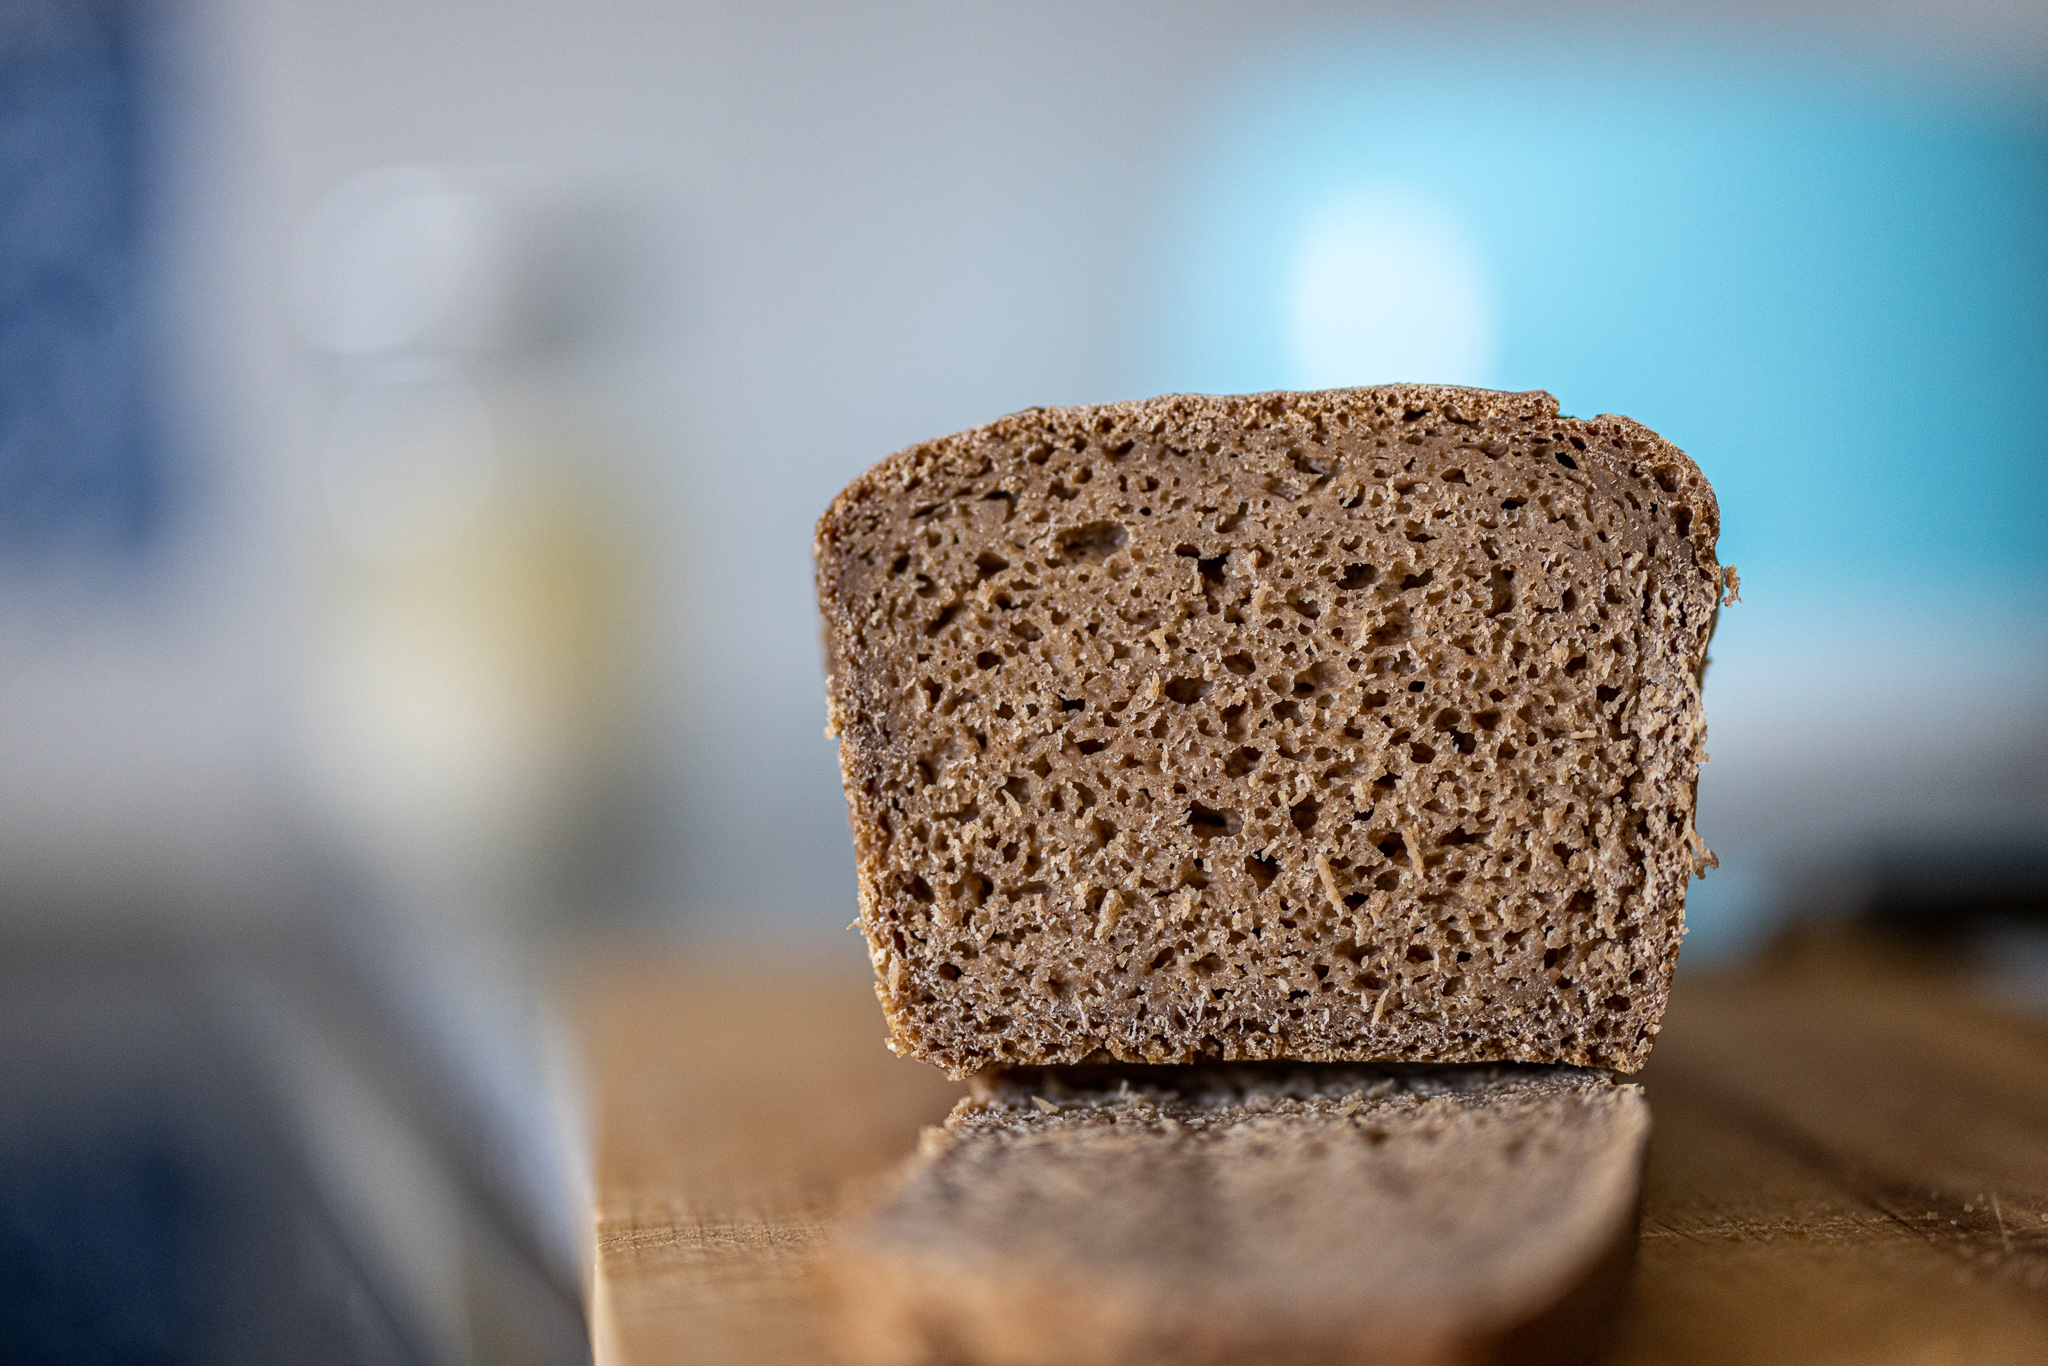
\includegraphics[width=\textwidth]{crumb}
  \caption{The crumb structure of rye bread. By making a wetter
  dough, more water evaporates during the baking and thus the
  crumb tends to be a bit more open. Generally, rye
  bread is never as fluffy as wheat sourdough bread. The crust
  of this bread is a bit pale. The crust color can be controlled
  by baking the bread for a longer period.}%
  \label{fig:rye-crumb}
\end{figure}

Carefully spread the dough with a spatula in your loaf pan. You
can wet the spatula to make this process easier. Spread it
until the surface looks smooth and shiny.

For proofing, I~recommend waiting around 60 minutes. An extended
proofing period does not make sense unless you want to further
increase the dough's acidity. The dough will not become fluffier
the longer you proof. With the short proofing period, however,
the dough will become a bit more homogenous. This way the final
bread looks more uniform. The proofing period also allows the
dough to fully extend and fill the edges of the loaf pan. I~also
like to move the dough to the fridge for proofing. The dough stays
good in the fridge for weeks. You can proceed and bake it at a
convenient time for you. 

Once you are happy with the proofing stage, proceed and bake your dough
just like you'd normally do. For more details please refer to 
Chapter~\ref{chapter:baking}. One challenging aspect
of using a loaf pan is to make sure that the center part of your
dough is properly cooked. For this reason, it is best to use a thermometer
and measure the internal temperature. The bread is
ready once the internal temperature reaches 92°C (197°F). I~recommend
removing the bread from the loaf pan once it reaches the desired
temperature. Then you can continue baking the loaf without the pan and
steam. This way you achieve a great crust all around your
loaf. You can bake as long as you like until you have achieved
your crust color of choice. The darker, the more crunchy
the crust and the more flavor it offers. If you feel your
dough might have been overly acidic, you can extend the baking time.
The longer you bake, the more acidity will evaporate.

This is one of my favorite breads to bake which I~eat on an
almost daily basis. The effort required to make bread like
this is much lower compared to a wheat-based dough. In some
cases, I~extend the recipe and add additional sourdough discard
to the dough. You can add as much discard as you like. The resulting
bread has a very complex but delicious flavor profile.
